
\section{Partioparaati 28.4.}

\vspace*{-0.64cm}
\begin{multicols}{2}

	\begin{center}
		\noindent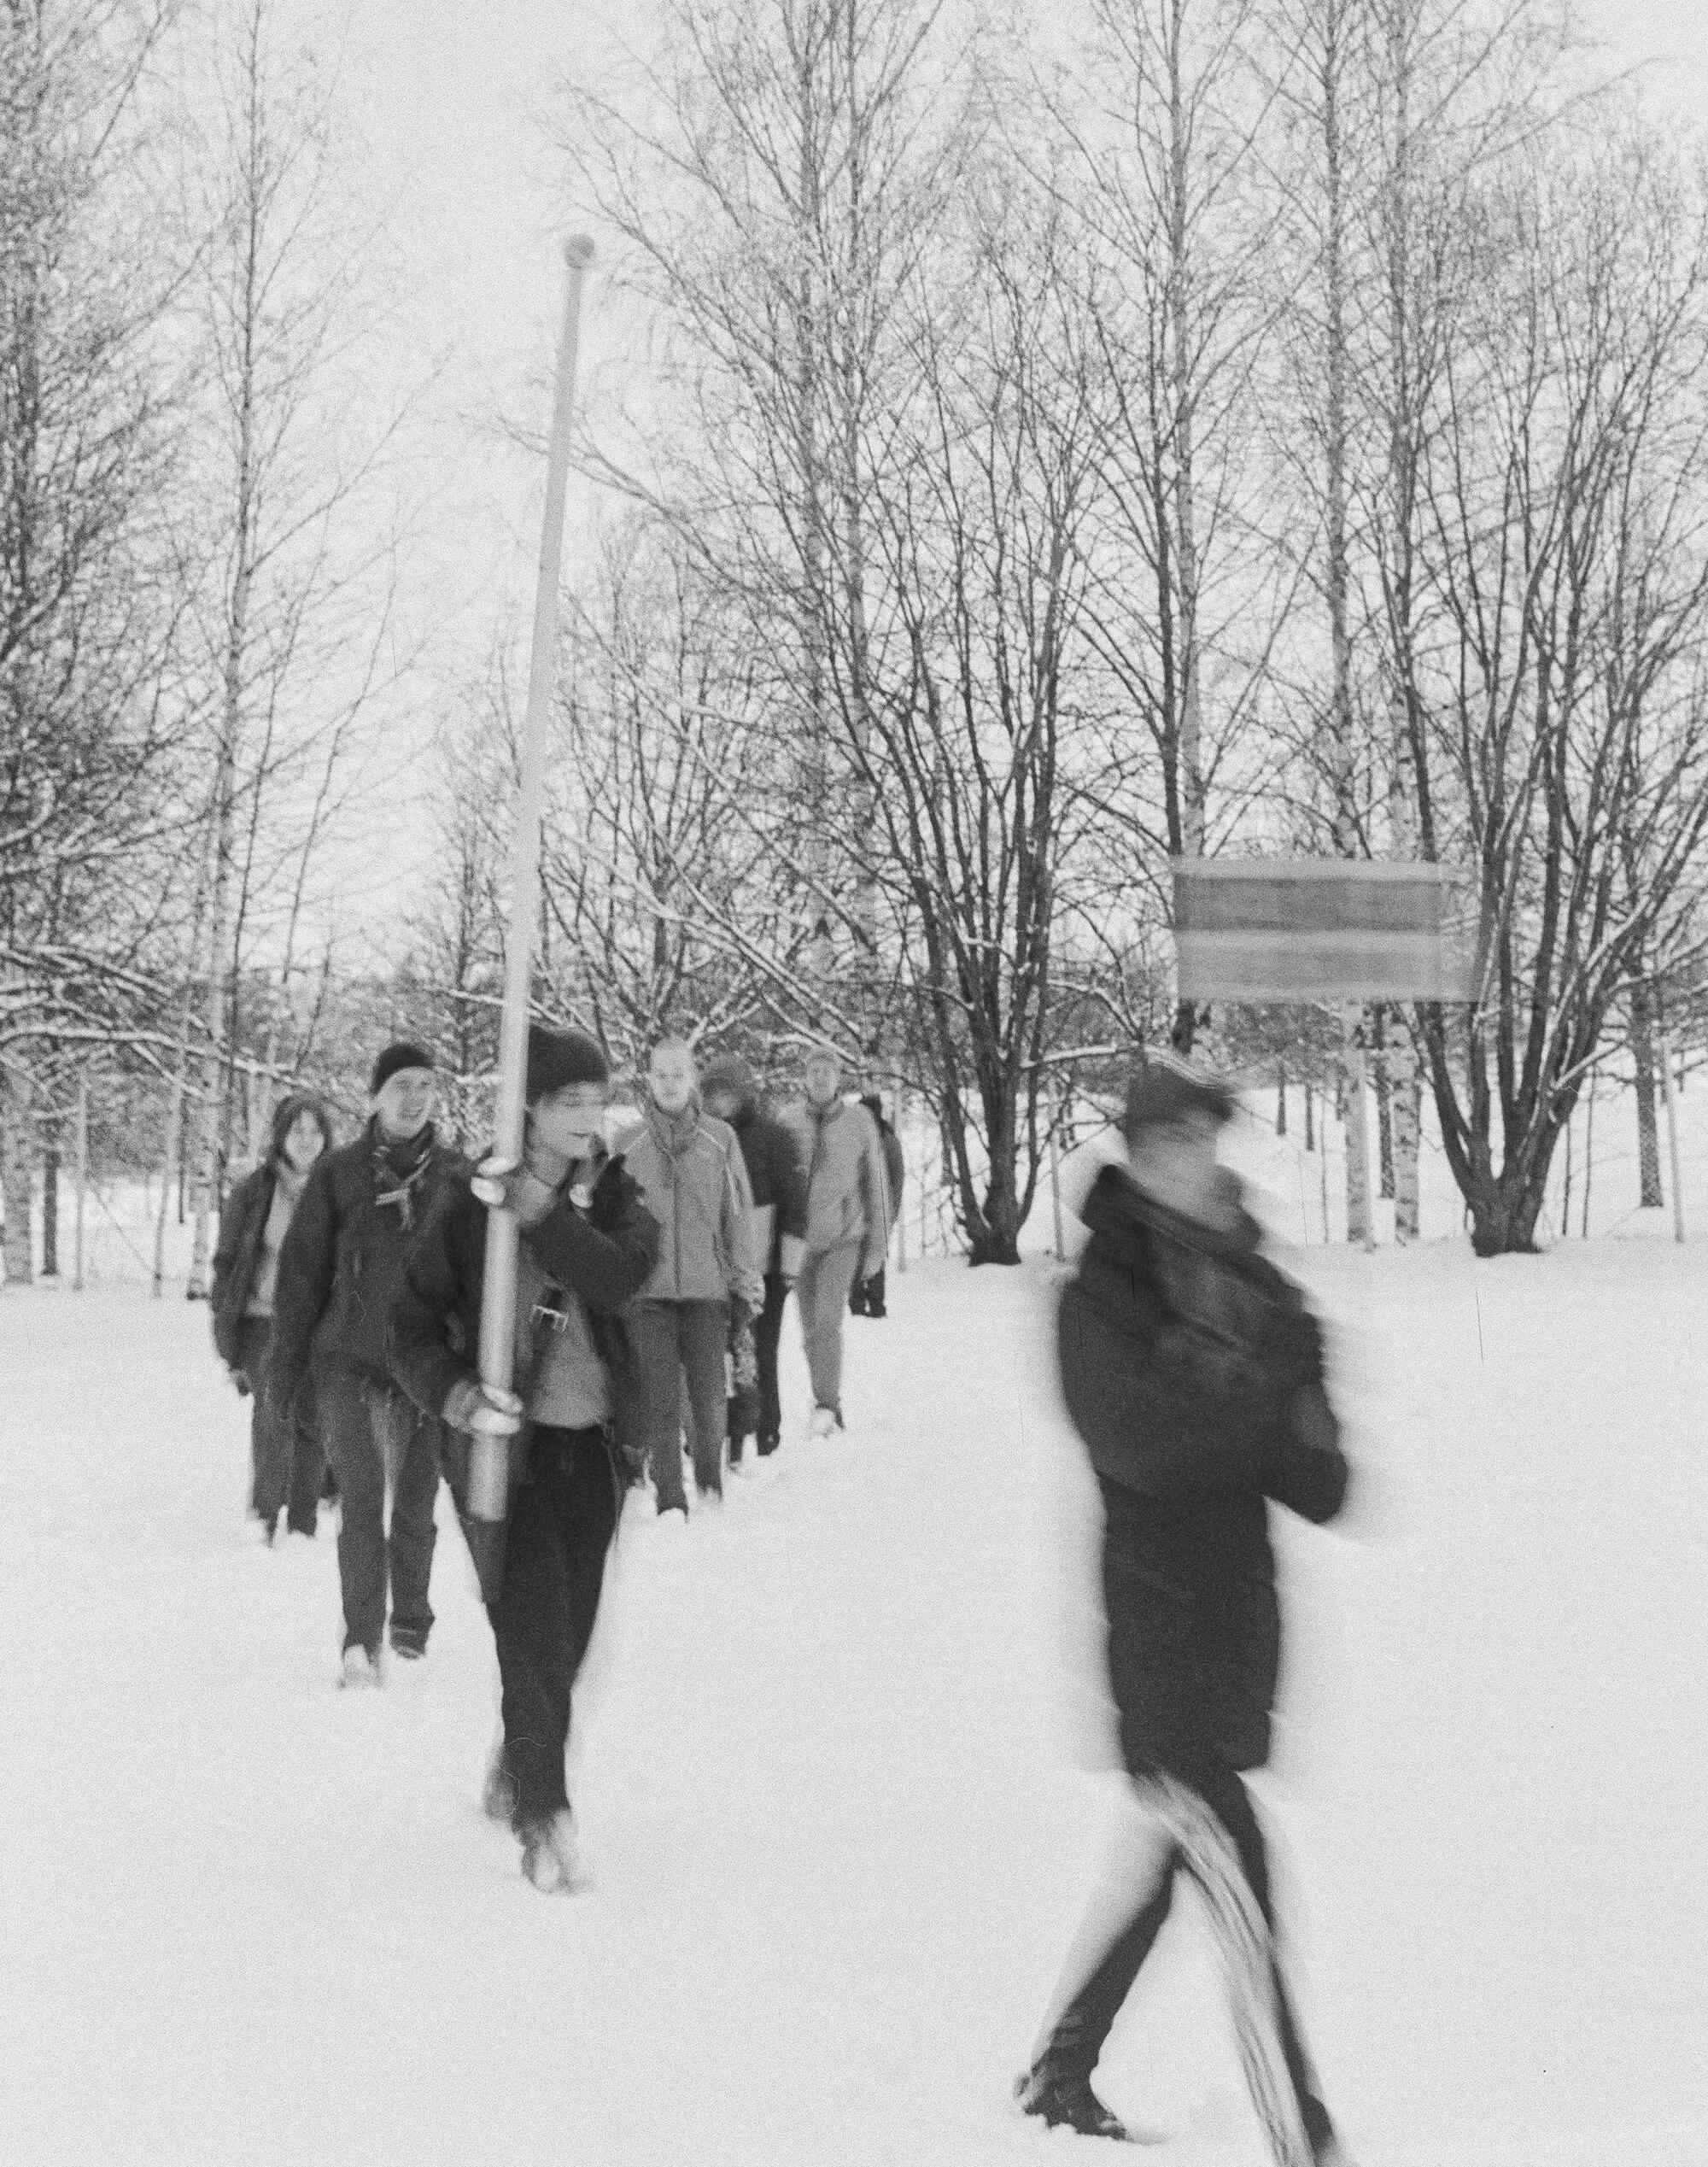
\includegraphics[width=0.85\linewidth]{assets/paraati1}
	\end{center}

	\vspace*{-0.32cm}
	\small\noindent KuRu:n paraatiosasto harjoiteli \mbox{paraati}protokollaa
	viikkokokouksessaan vielä talvisessa säässä\ldots

	\columnbreak

	\begin{center}
		\noindent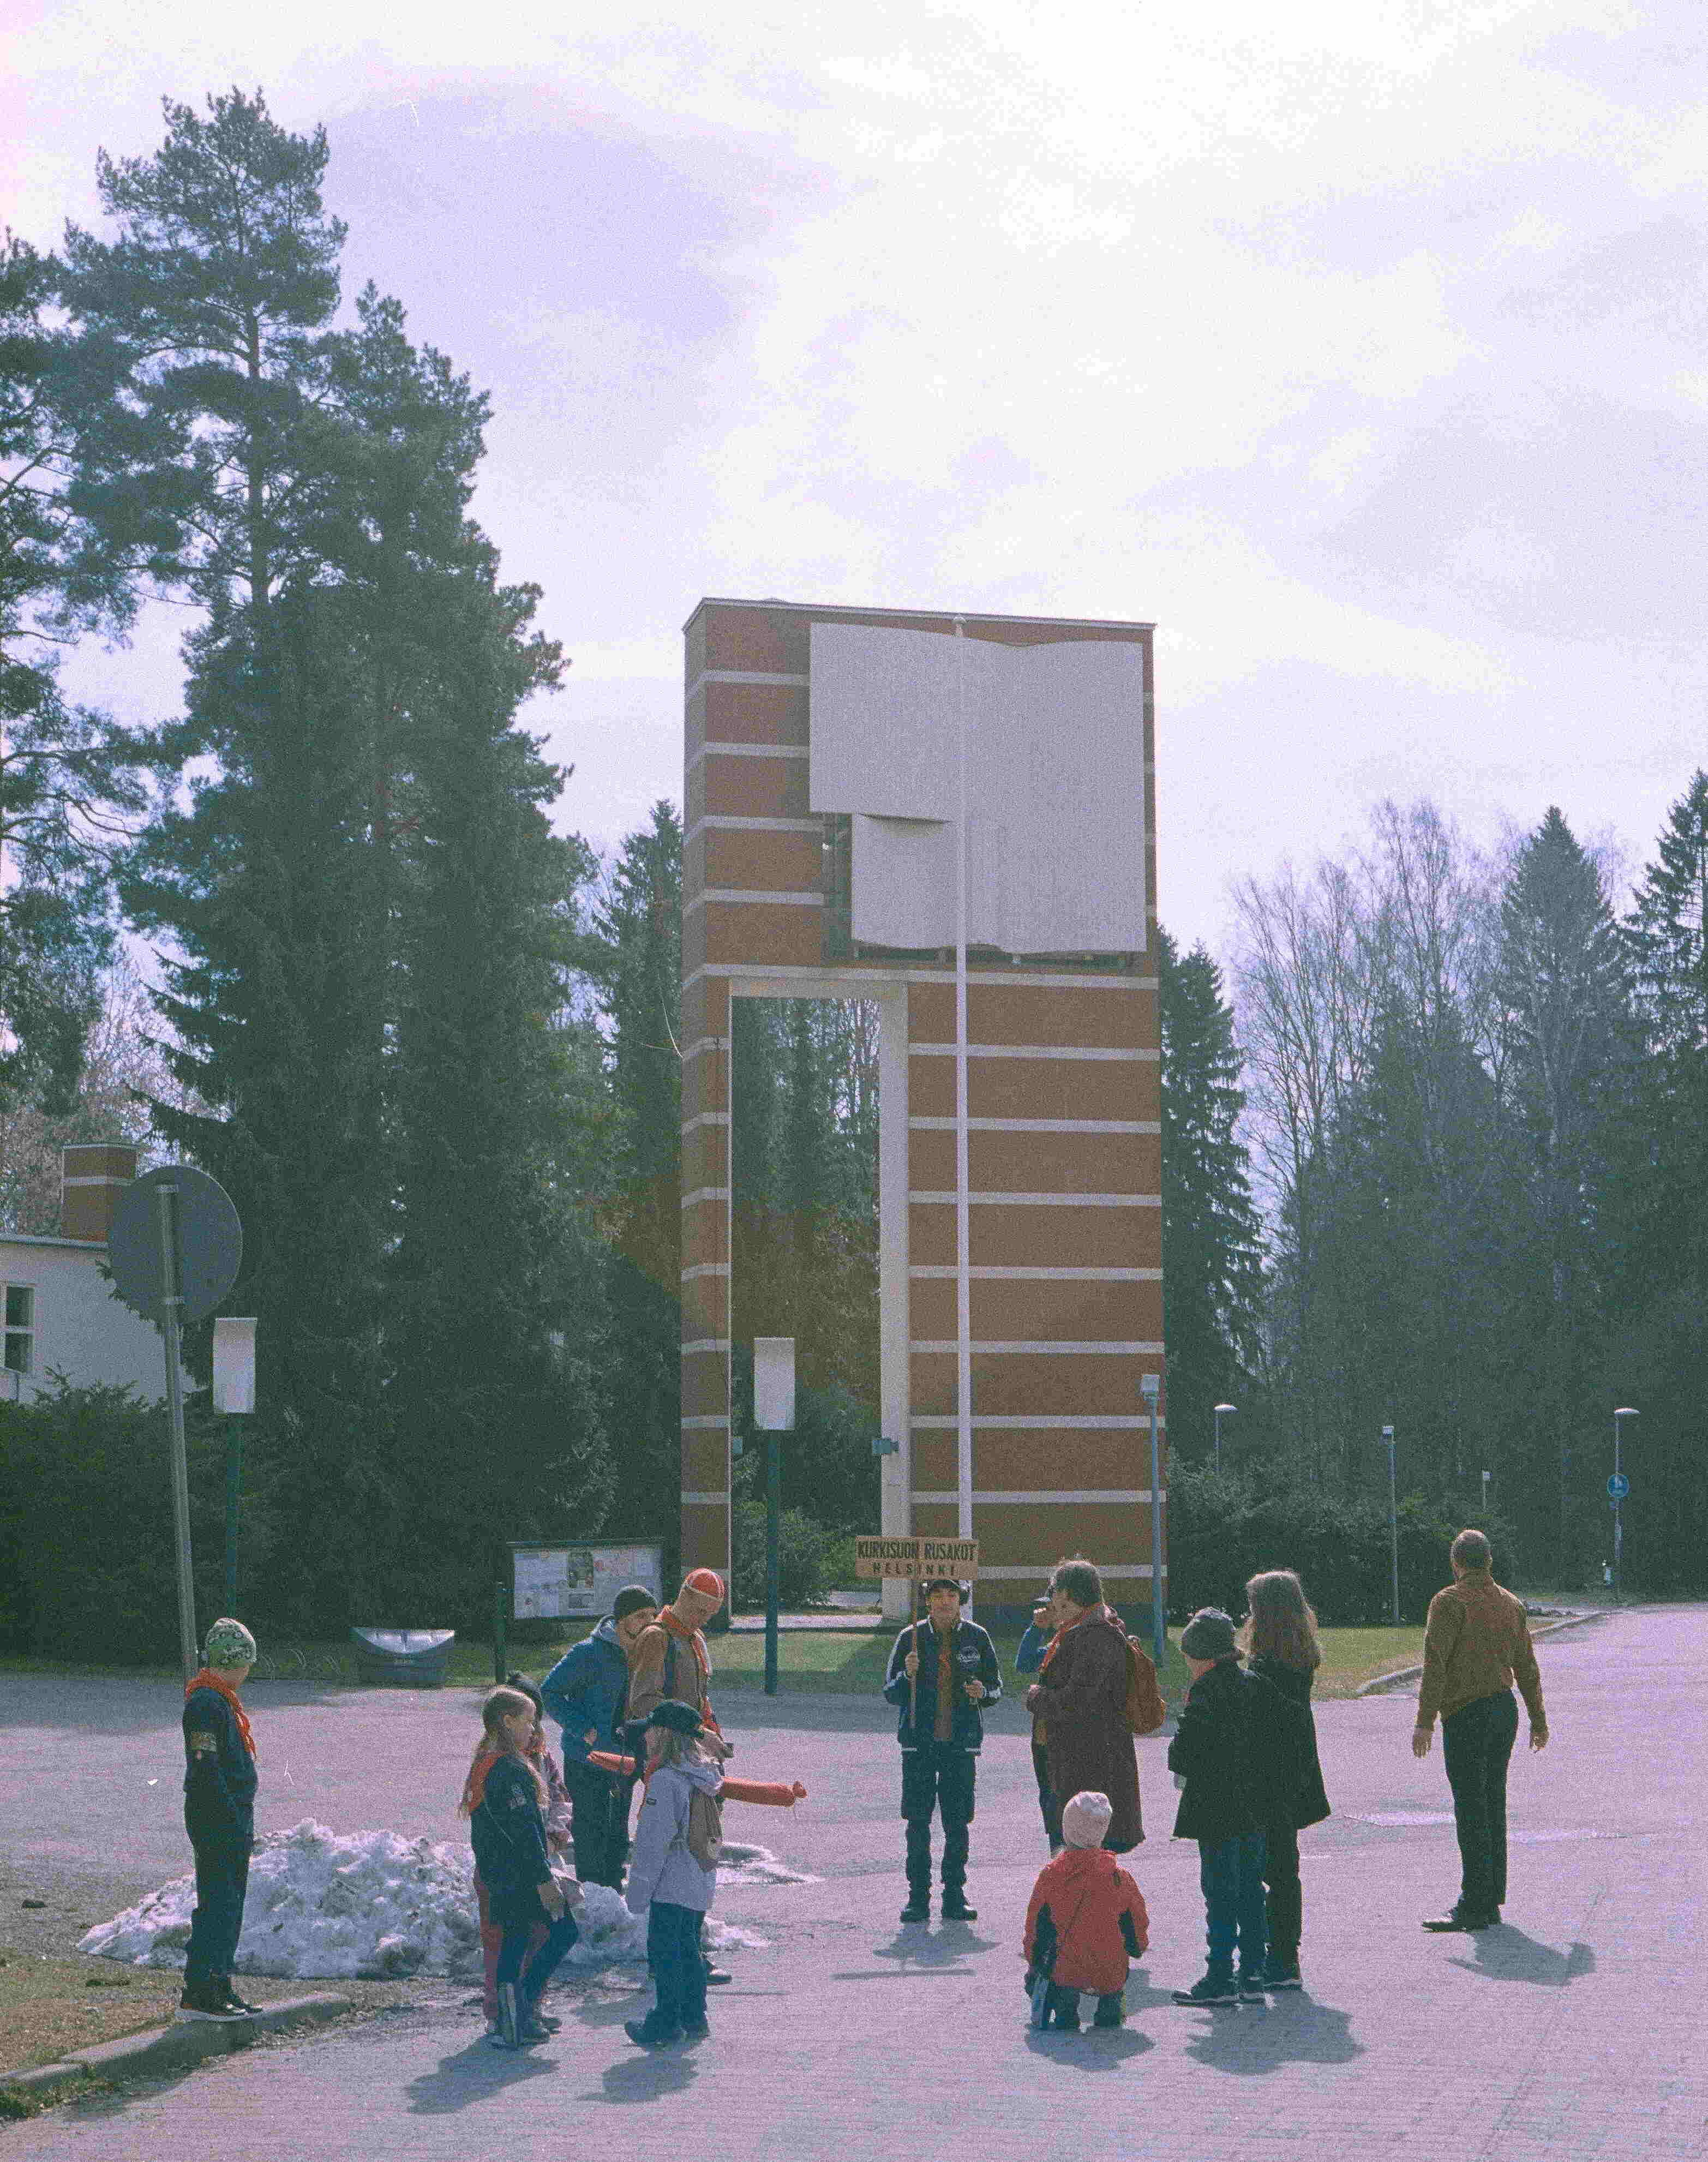
\includegraphics[width=0.85\linewidth]{assets/paraati2}
	\end{center}

	\vspace*{-0.32cm}
	\ldots ja pari päivää myöhemmin kokoontui keväisessä kelissä ja matkusti kohti keskustaa.

\end{multicols}
\begin{multicols}{2}

	\begin{center}
		\noindent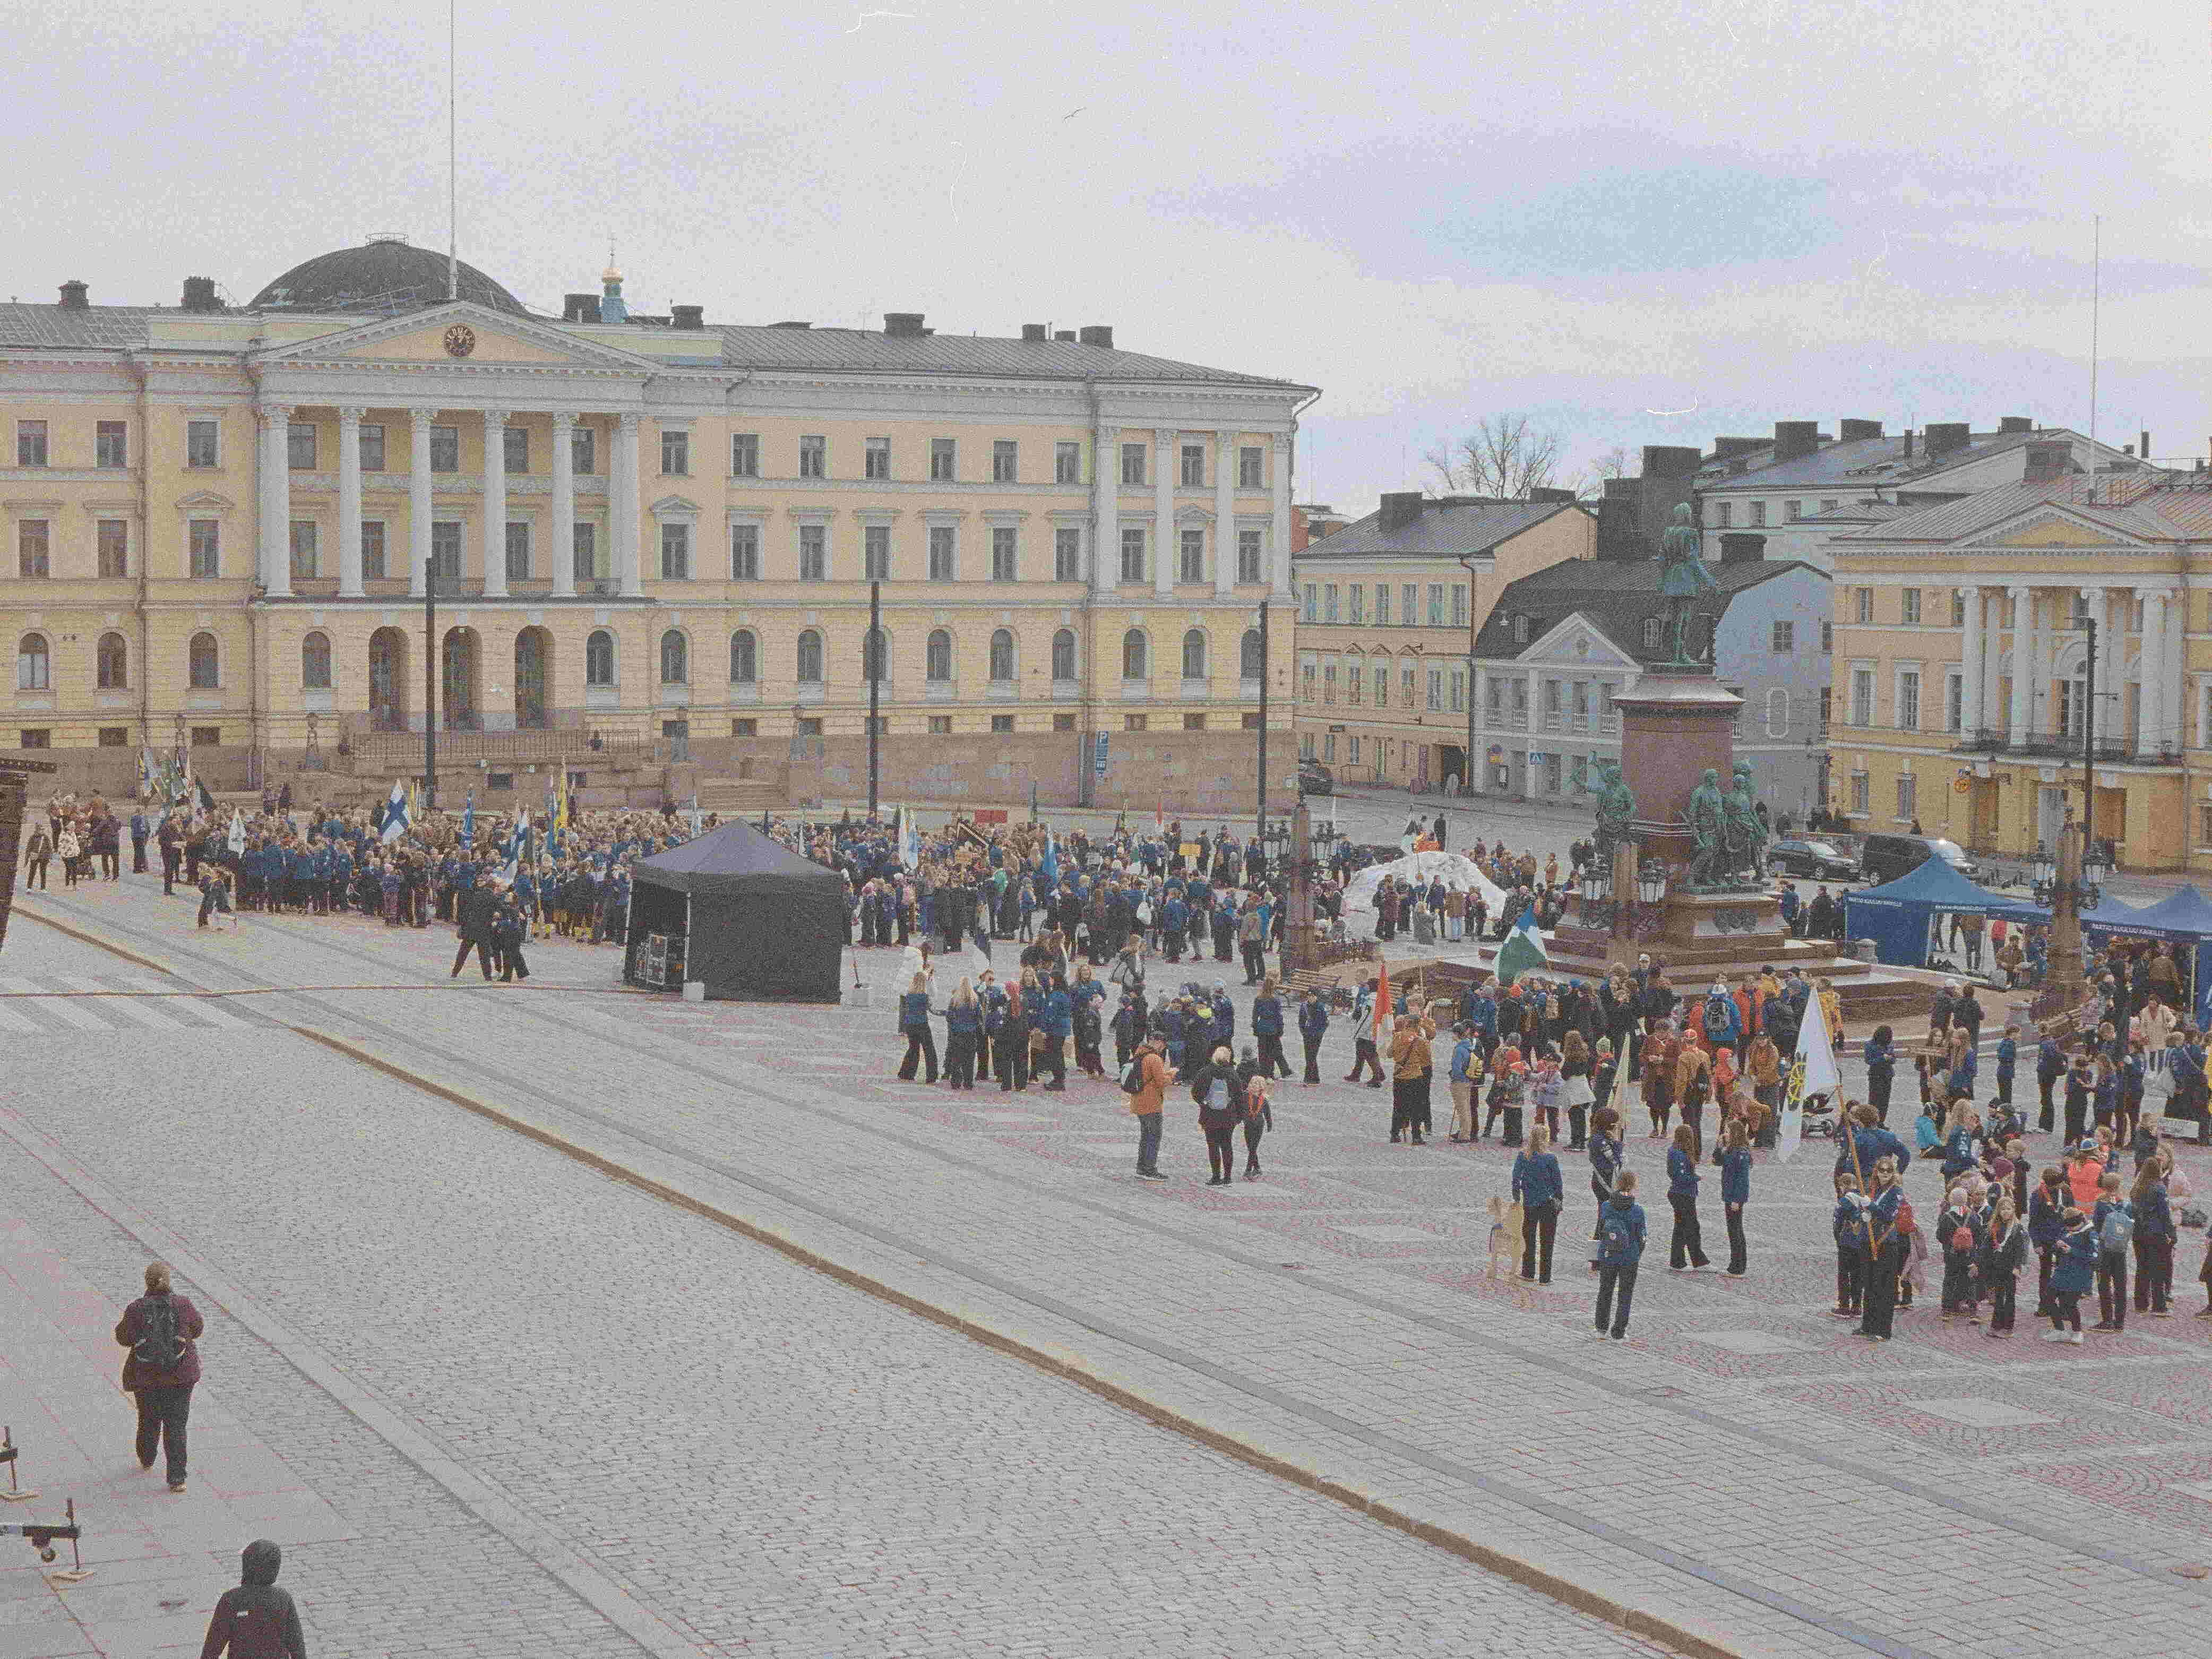
\includegraphics[width=0.85\linewidth]{assets/paraati4}
	\end{center}

	\vspace*{-0.16cm}
	\small Senaatintorilta löytyi yli kaksi tuhatta partiolaista Helsingistä, Espoosta, Vantaalta ja Kauniaisista. Siellä marsittiin, nautitiin musiikista ja ajoittain auringosta.

	Paraatin päätteeksi KuRu:n osasto sai vielä maistuvan lounaan läheisessä \mbox{pitseriassa}!

	\columnbreak

	\begin{center}
		\noindent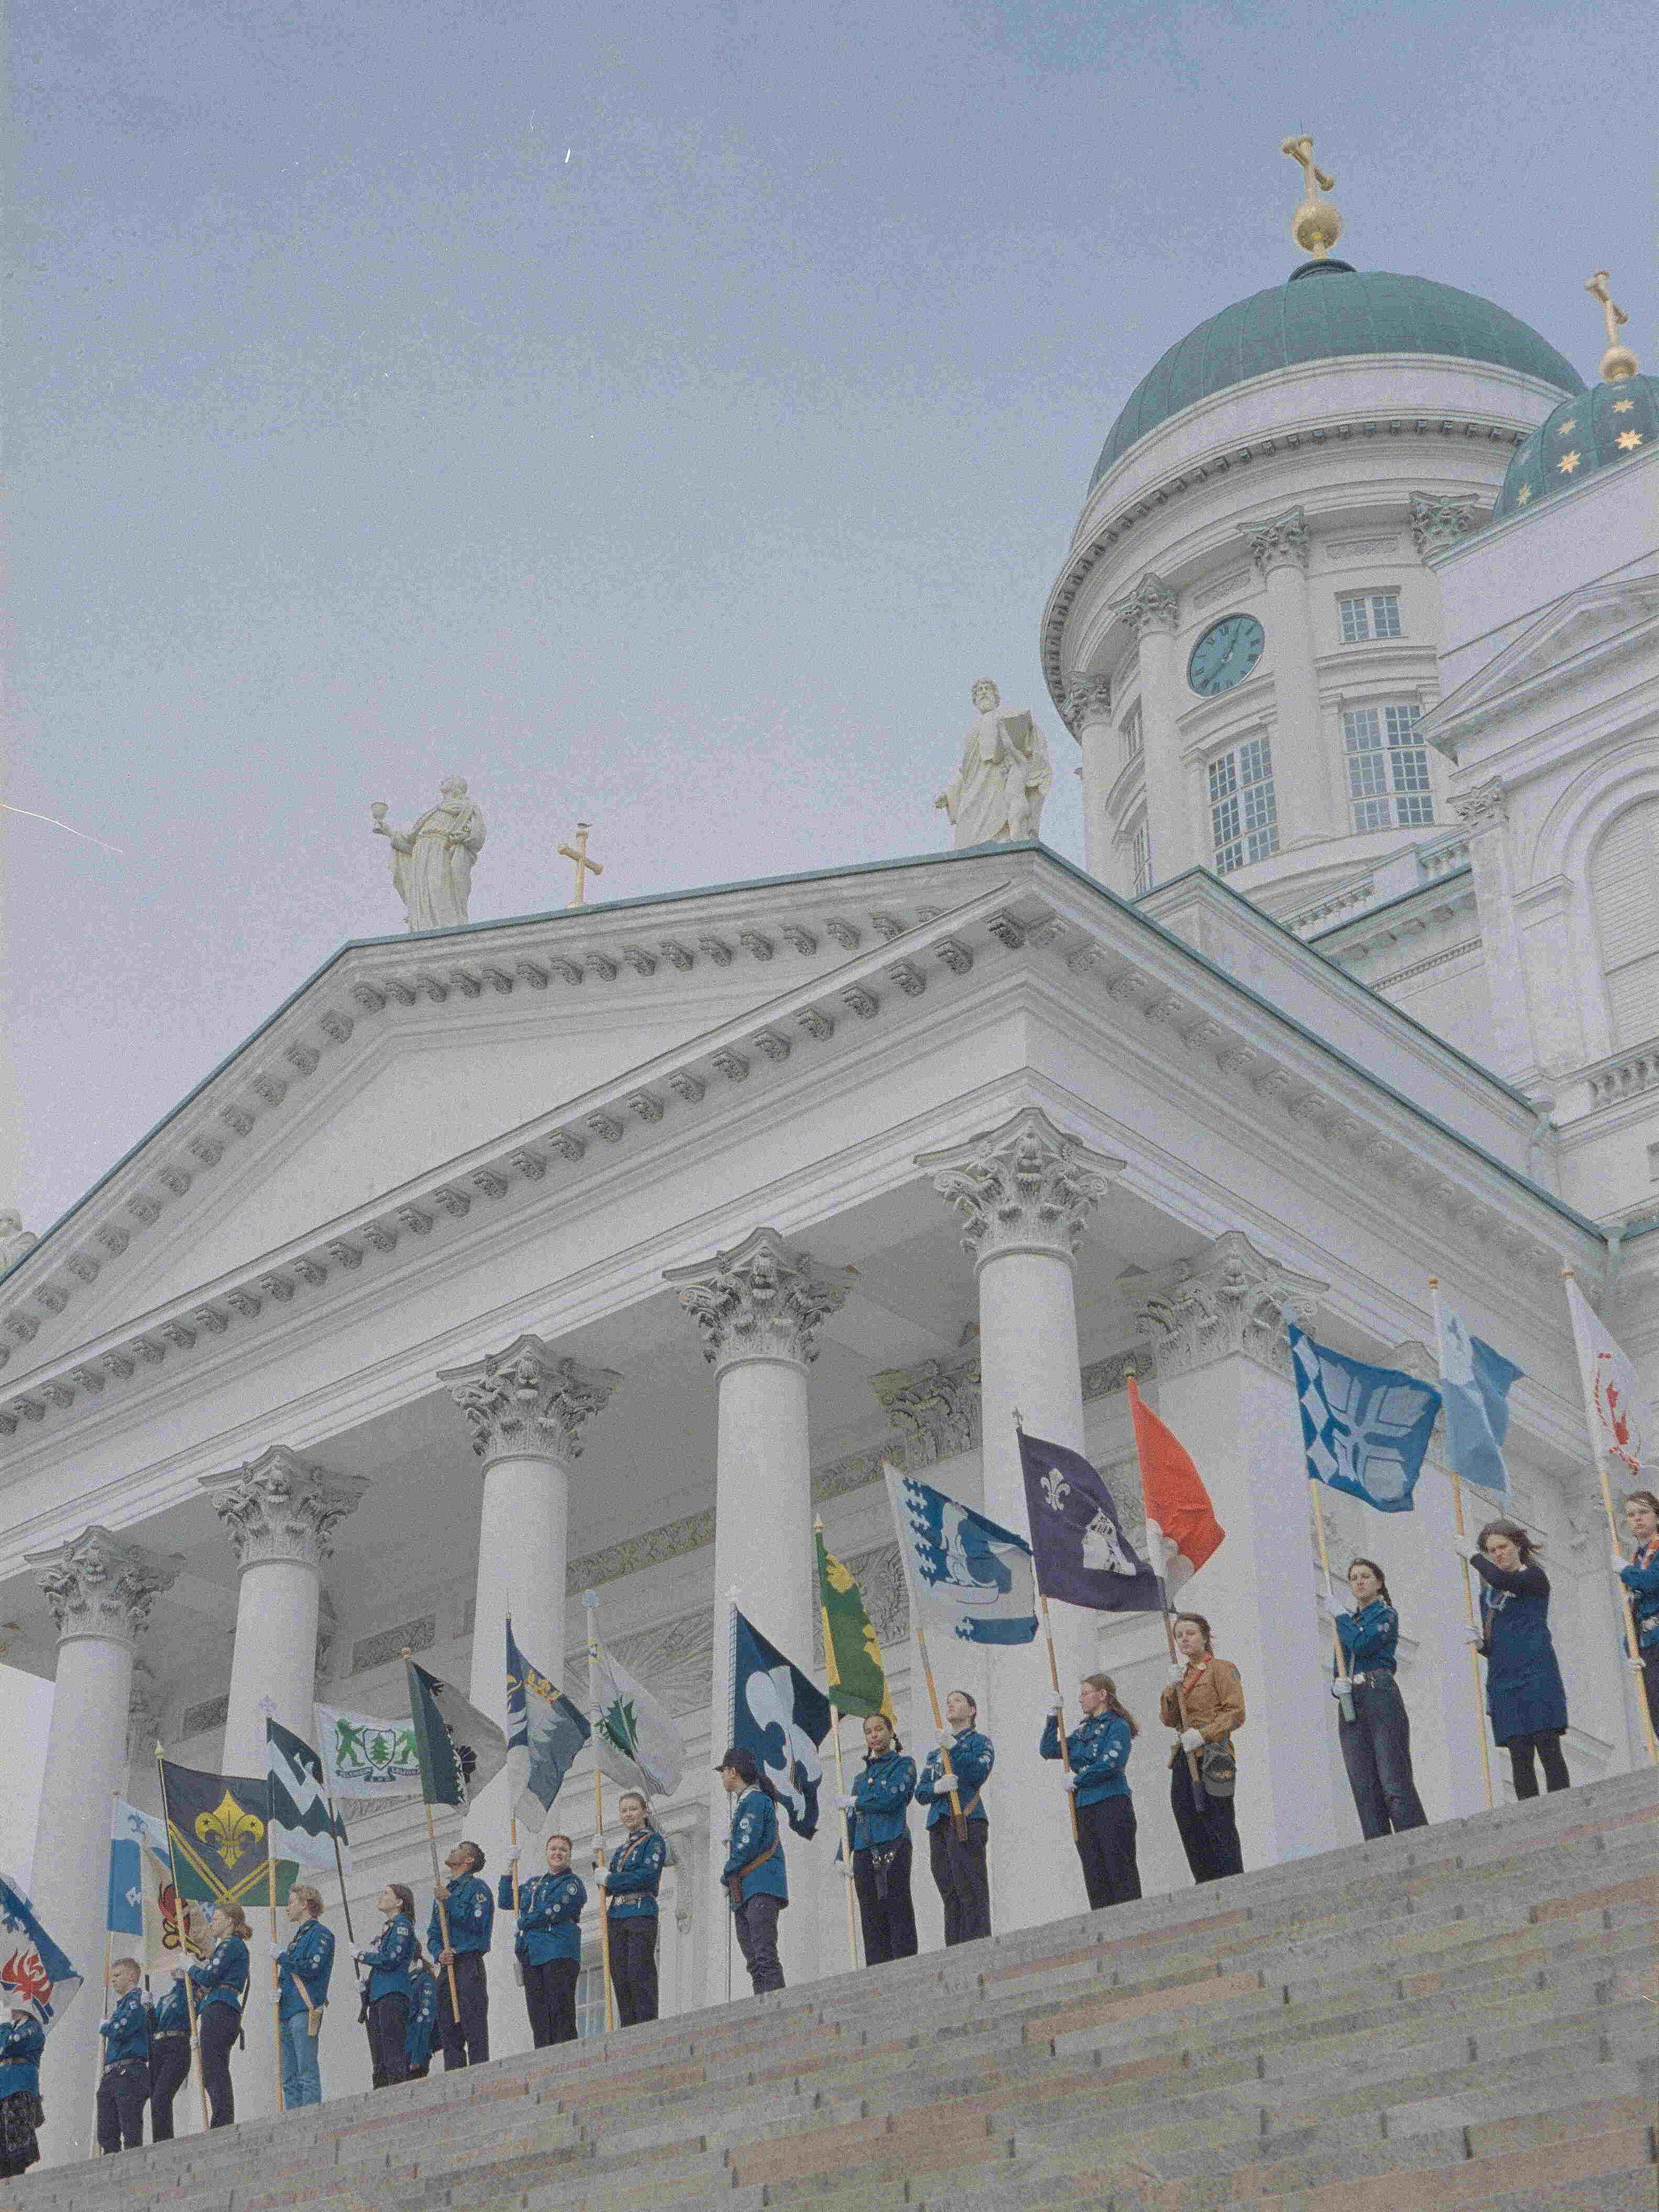
\includegraphics[width=0.85\linewidth]{assets/paraati3}
	\end{center}


\end{multicols}

% \vspace*{-0.32cm}

\medskip
\noindent\null\hfill Tanguy Gérôme
